\chapter{Исследовательский раздел}

В данном разделе представлены эксперименты для проведения сравнительного анализа быстродействия реализуемых алгоритмов синтеза изображения.

\section{Постановка эксперимента}

В эксперименте исследуется зависимость времени выполнения алгоритмов синтеза изобржения в зависимости от количества объектов сцены при двух и пяти различных источниках освещения.

При проведении эксперимента все объекты сцены будут расположены в поле зрения камеры, чтобы исключить случаи, когда реальная отрисовка объекта не выполняется.

Количество объектов сцены будет варьироваться от 1 по 7 с шагом 2.

Для каждого случая будет рассчитано время синтеза изображения алгоритмом предобработки (быстрая отрисовка) и алгоритмом трассировки лучей.

Полученный результат не усредняется.

\section{Технические характеристики}

Ниже приведены характеристики устройства, на котором будет производиться эксперимент:

\begin{itemize}
    \item операционная система: Pop!\_OS 21.04 \cite{pop} Linux 64-bit;
    \item оперативная память: 8Gb;
    \item процессор: Intel Core i7-8750H @ 12x 4.1 GHz.
\end{itemize}

\section{Результаты эксперимента}

Ниже в таблице \ref{exp:res} представлены результаты эксперимента.

\begin{table}[h]
	\caption{Время работы алгоритмов при различных параметрах сцены}
	\begin{center}
		\begin{tabular}{|c|c|c|c|}
			\hline
			\specialcell{кол-во объектов \\ в сцене} &
			\specialcell{кол-во источников \\ освещения} &
			\specialcell{время \\ закраски} &
			\specialcell{время \\ трассировки} \\
			\hline
			1 & 2 & 10.3 мс & 10.5 с \\
			\hline
			3 & 2 & 12.2 мс & 25.7 с \\
			\hline
			5 & 2 & 15.4 мс & 107 с \\
			\hline
			7 & 2 & 31.5 мс & 174 с \\
			\hline
			1 & 5 & 10.3 мс & 14.8 с \\
			\hline
			3 & 5 & 13.7 мс & 62.1 с \\
			\hline
			5 & 5 & 15.9 мс & 334 с \\
			\hline
			7 & 5 & 35.8 мс & 1520 с \\
			\hline
		\end{tabular}
	\end{center}
	\label{exp:res}
\end{table}

\begin{figure}[h]
	\centering
	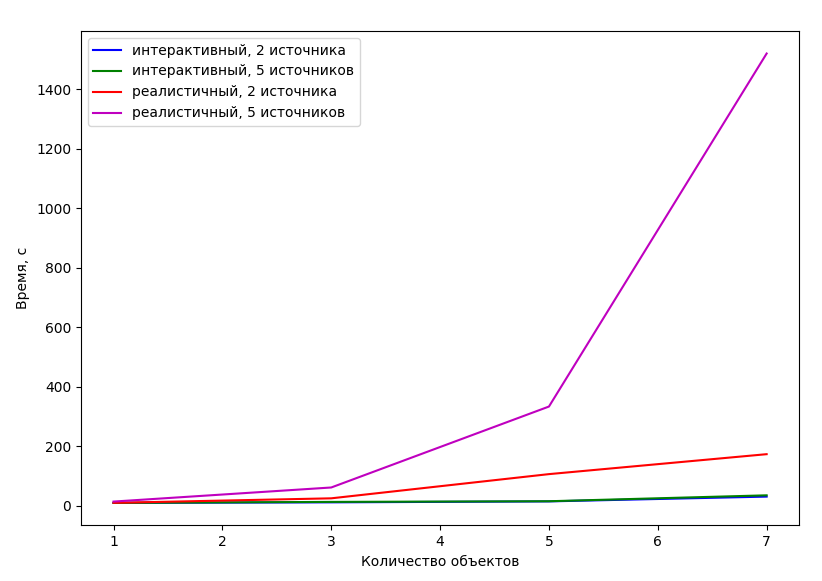
\includegraphics[width=0.7\linewidth]{inc/img/graph}
	\caption{Время работы алгоритмов при различных параметрах сцены}
	\label{fig:graph}
\end{figure}


Как видно из рисунка \ref{fig:graph}, время затрачиваемое на отрисовку с использованием трассировки лучей в тысячу раз превосходит время затрачиваемое быстрым алгоритмом.

\section{Вывод}

В данном разделе был поставлен эксперимент по сравнению производительности интерактивного и реалистичного режимов синтеза изображения в разработанном ПО при различных параметрах сцены.

Количество источников освещения незначительно влияет на время при быстрой закраске, при методе трассировки лучей на порядок увеличивает время синтеза изображения.

По результатам эксперимента было выявлено, что интерактивный режим выгодно использовать при настройке параметров сцены для дальнейшего синтеза реалистичного изображения, время получение которого в тысячи раз превышает время отрисовки в интерактивном режиме.
